\begin{tikzpicture}[remember picture,overlay]
    \node[
    anchor=south west,
    inner sep=0pt,
    outer sep=0pt
    ] at (current page.south west) {%
        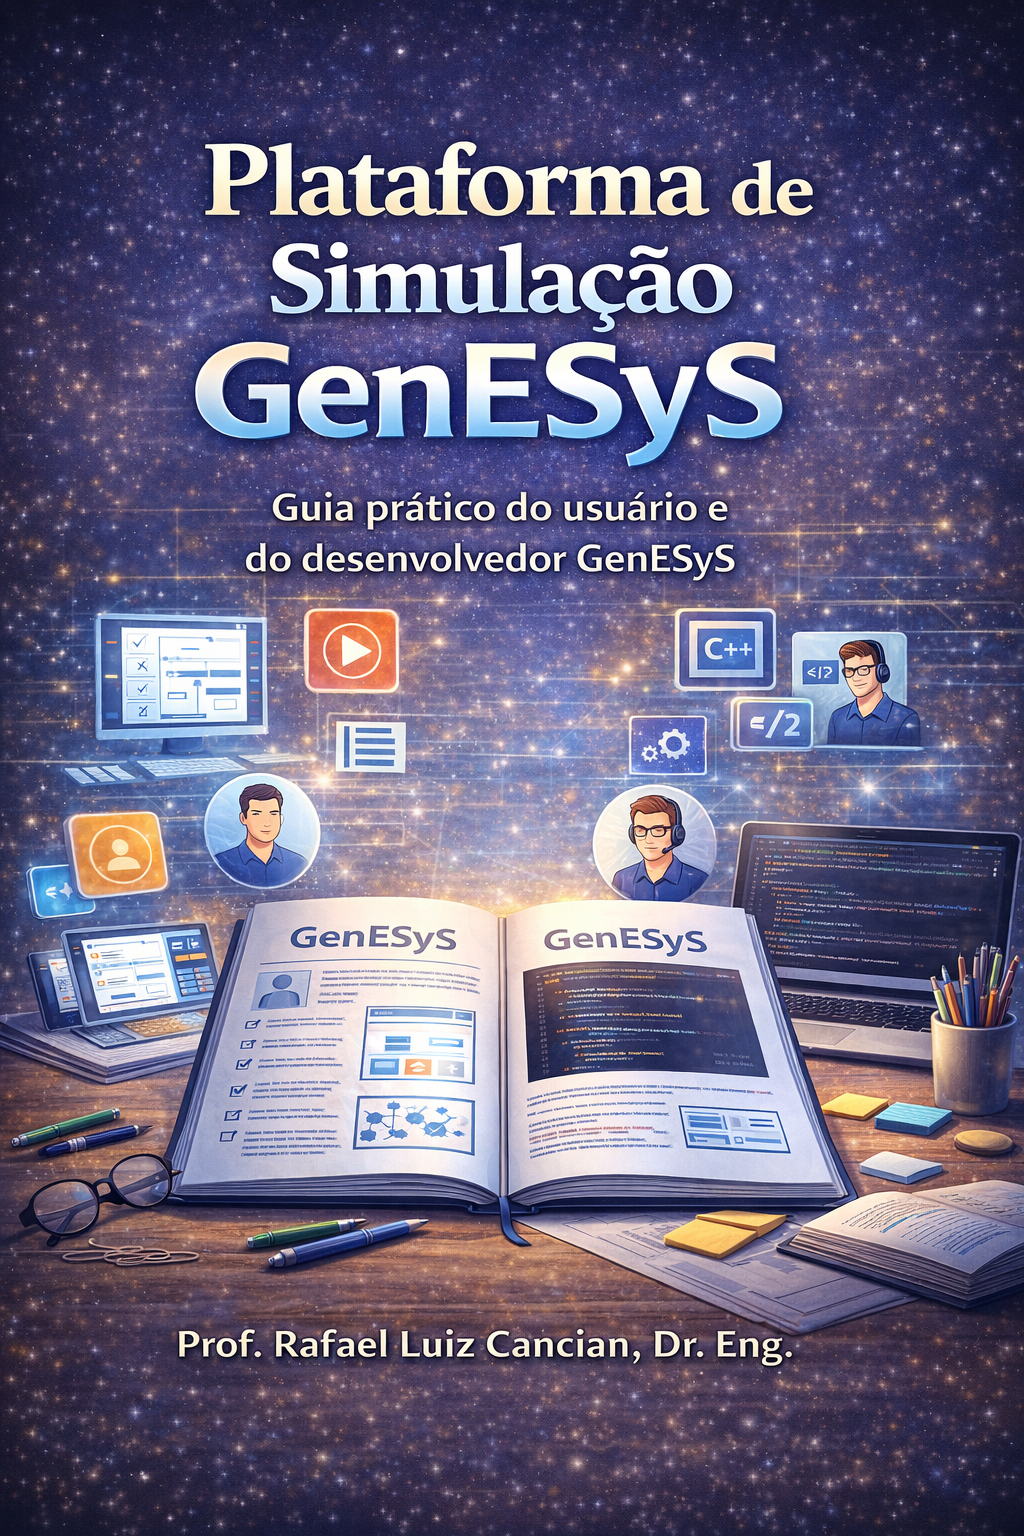
\includegraphics[width=\paperwidth,height=\paperheight]{figs/capa.png}%
    };
\end{tikzpicture}

%\begin{tikzpicture}[remember picture,overlay]
%	\node[inner sep=0pt] (background) at (current page.center) {\safeincludegraphics[width=\paperwidth]{figs/background}};
%	\draw (current page.center) node [fill=ocre,fill opacity=0.15,text opacity=1,inner sep=0.25cm] {
%		% list of font families: https://tex.stackexchange.com/questions/378623/how-can-i-get-a-list-of-all-fontfamily-fontseries-combinations
%		\Huge\centering\bfseries\sffamily\parbox[c][][t]{\paperwidth} {
%			\vspace{5mm}
%			\color{black} \centering
%			%\vspace{30mm}%30
%			{\fontsize{35}{20}
%			%	\fontfamily{nightmare-codehack}\selectfont
%				\fontfamily{put}\selectfont
%				\mycontour{Modelagem e}{3.0}{white}\\
%				\mycontour{Simulação de Sistemas}{3.0}{white}
%			}\\
%			%\centering
%			%\safeincludegraphics[width=0.8\linewidth]{figs/titulo_livro}
%
%			\vspace{6mm}%85%60
%			%\color{black}
%			{\Large
%				%\mycontour{Apostila de aula de}{0.85}{white}\\
%				\mycontour{Métodos, práticas e fundamentos para o}{0.85}{white}\\
%				%\vspace{-0.3cm}
%				\mycontour{desenvolvimento e uso de modelos e}{0.85}{white}\\
%				\vspace{-0.45cm}
%				\mycontour{estudos científicos de simulação}{0.85}{white}}\\
%
%			\vspace{64mm}%6  % alinhamento centrado na página
%
%			{\Large
%				\mycontour{Exemplos práticos de uso com}{0.65}{ocre!30}\\
%				\vspace{-0.1cm}
%				\mycontour{Scilab/xCos, Ptolemy II, OpenModellica,}{0.65}{ocre!30}\\
%				\vspace{-0.1cm}
%				%\mycontour{OpenModelica, Arena e GenESyS}{0.65}{ocre!30}\\
%				\mycontour{Arena e GenESyS}{0.65}{ocre!30}\\
%				%\vspace{-0.1cm}
%				%{\large \mycontour{(com código-fonte aberto, disponível e comentado)}{0.65}{ocre!30}}\\
%			}
%
%
%			%\mycontour{engenheiros e cientistas da computação}{0.85}{white}}\\
%
%			\color{white}
%			%{\large \mycontour{(Inclui exemplos em Simulink, Octave, OpenModelica, C++ e Arena, com aplicações em}{0.35}{ocre}}\\
%			%{\large \mycontour{sistemas embarcados e cyber-físicos, bioquímicos e genéticos, e de controle e automação)}{0.35}{ocre}}\\
%			\vspace{17mm}
%			%\color{white}
%			{\large \mycontour{Edição INTERNA de RASCUNHO versão \numeroversaoapostila}{0.25}{ocre}}\\
%			\vspace{-0.4cm}
%			%{\large \mycontour{Compartlhamento proibido.}{0.25}{ocre}}\\
%			{\large \mycontour{TODOS OS DIREITOS RESERVADOS.%PROIBIDA A REPRODUÇÃO TOTAL OU PARCIAL.
%				}{0.25}{ocre}}\\
%			\vspace{9mm}
%			{\Large \mycontour{\pronomenomeautor}{0.25}{ocre}\\
%				\vspace{-0.5cm}
%				%\Large \mycontour{Prof\textsuperscript{a}. Dr\textsuperscript{a}. Eng. Maiara Heil Cancian}{0.25}{ocre}
%			}
%		}
%	};
%\end{tikzpicture}
%
